\section{Introduction}
In this chapter will be presented the architecture of CPIM especially for the NoSQL service as it was before this work, then will be explained how was possible to include Kundera as persistence layer for the NoSQL service in CPIM and what problem has been faced during the process.
Furthermore in section \ref{sec:hegira} is shown how the integration with the migration system \textit{Hegira} has been introduced, what are the feature supported by this integration and which design choices has been put in place. 

\section{CPIM architecture}
To be able to expose a common interface for the multiple services supported by the library, CPIM adopts heavily the factory and singleton patterns.

\noindent The main access point of the library is the \texttt{MF} (Manager Factory) a singleton object which is responsible of reading the configuration files and exposing a set of methods that will build instances for the service factories.
The initialization is done through the first call to \texttt{MF.getFactory()} which read the configuration files and build an instance of \texttt{CloudMetadata} which will be referenced by all the other services and contains all the information stored in the configuration files.
 
\newparagraph The library is organized in several packages each of one is responsible of a particular service.
\noindent Each service exposes a factory class which is invoked through the \texttt{MF} factory, the service factory maintains a singleton instance of the provider-specific service implementation which is built at the first call based on the configuration available inside the singleton instance of \texttt{CloudMetadata}.
The result of this process is that with the same method call, based on the configuration file, is instantiated one service implementation or another.

\subsection{NoSQL service}
Before this work CPIM library supports NoSQL interaction through Java Persistence API.
The interoperability with the supported clouds is made possible thanks to the previously described factory pattern, a complete class diagram for this service can be seen in the figure \ref{fig:cpim-nosql}.

\begin{figure}[tbh]
  \centering
  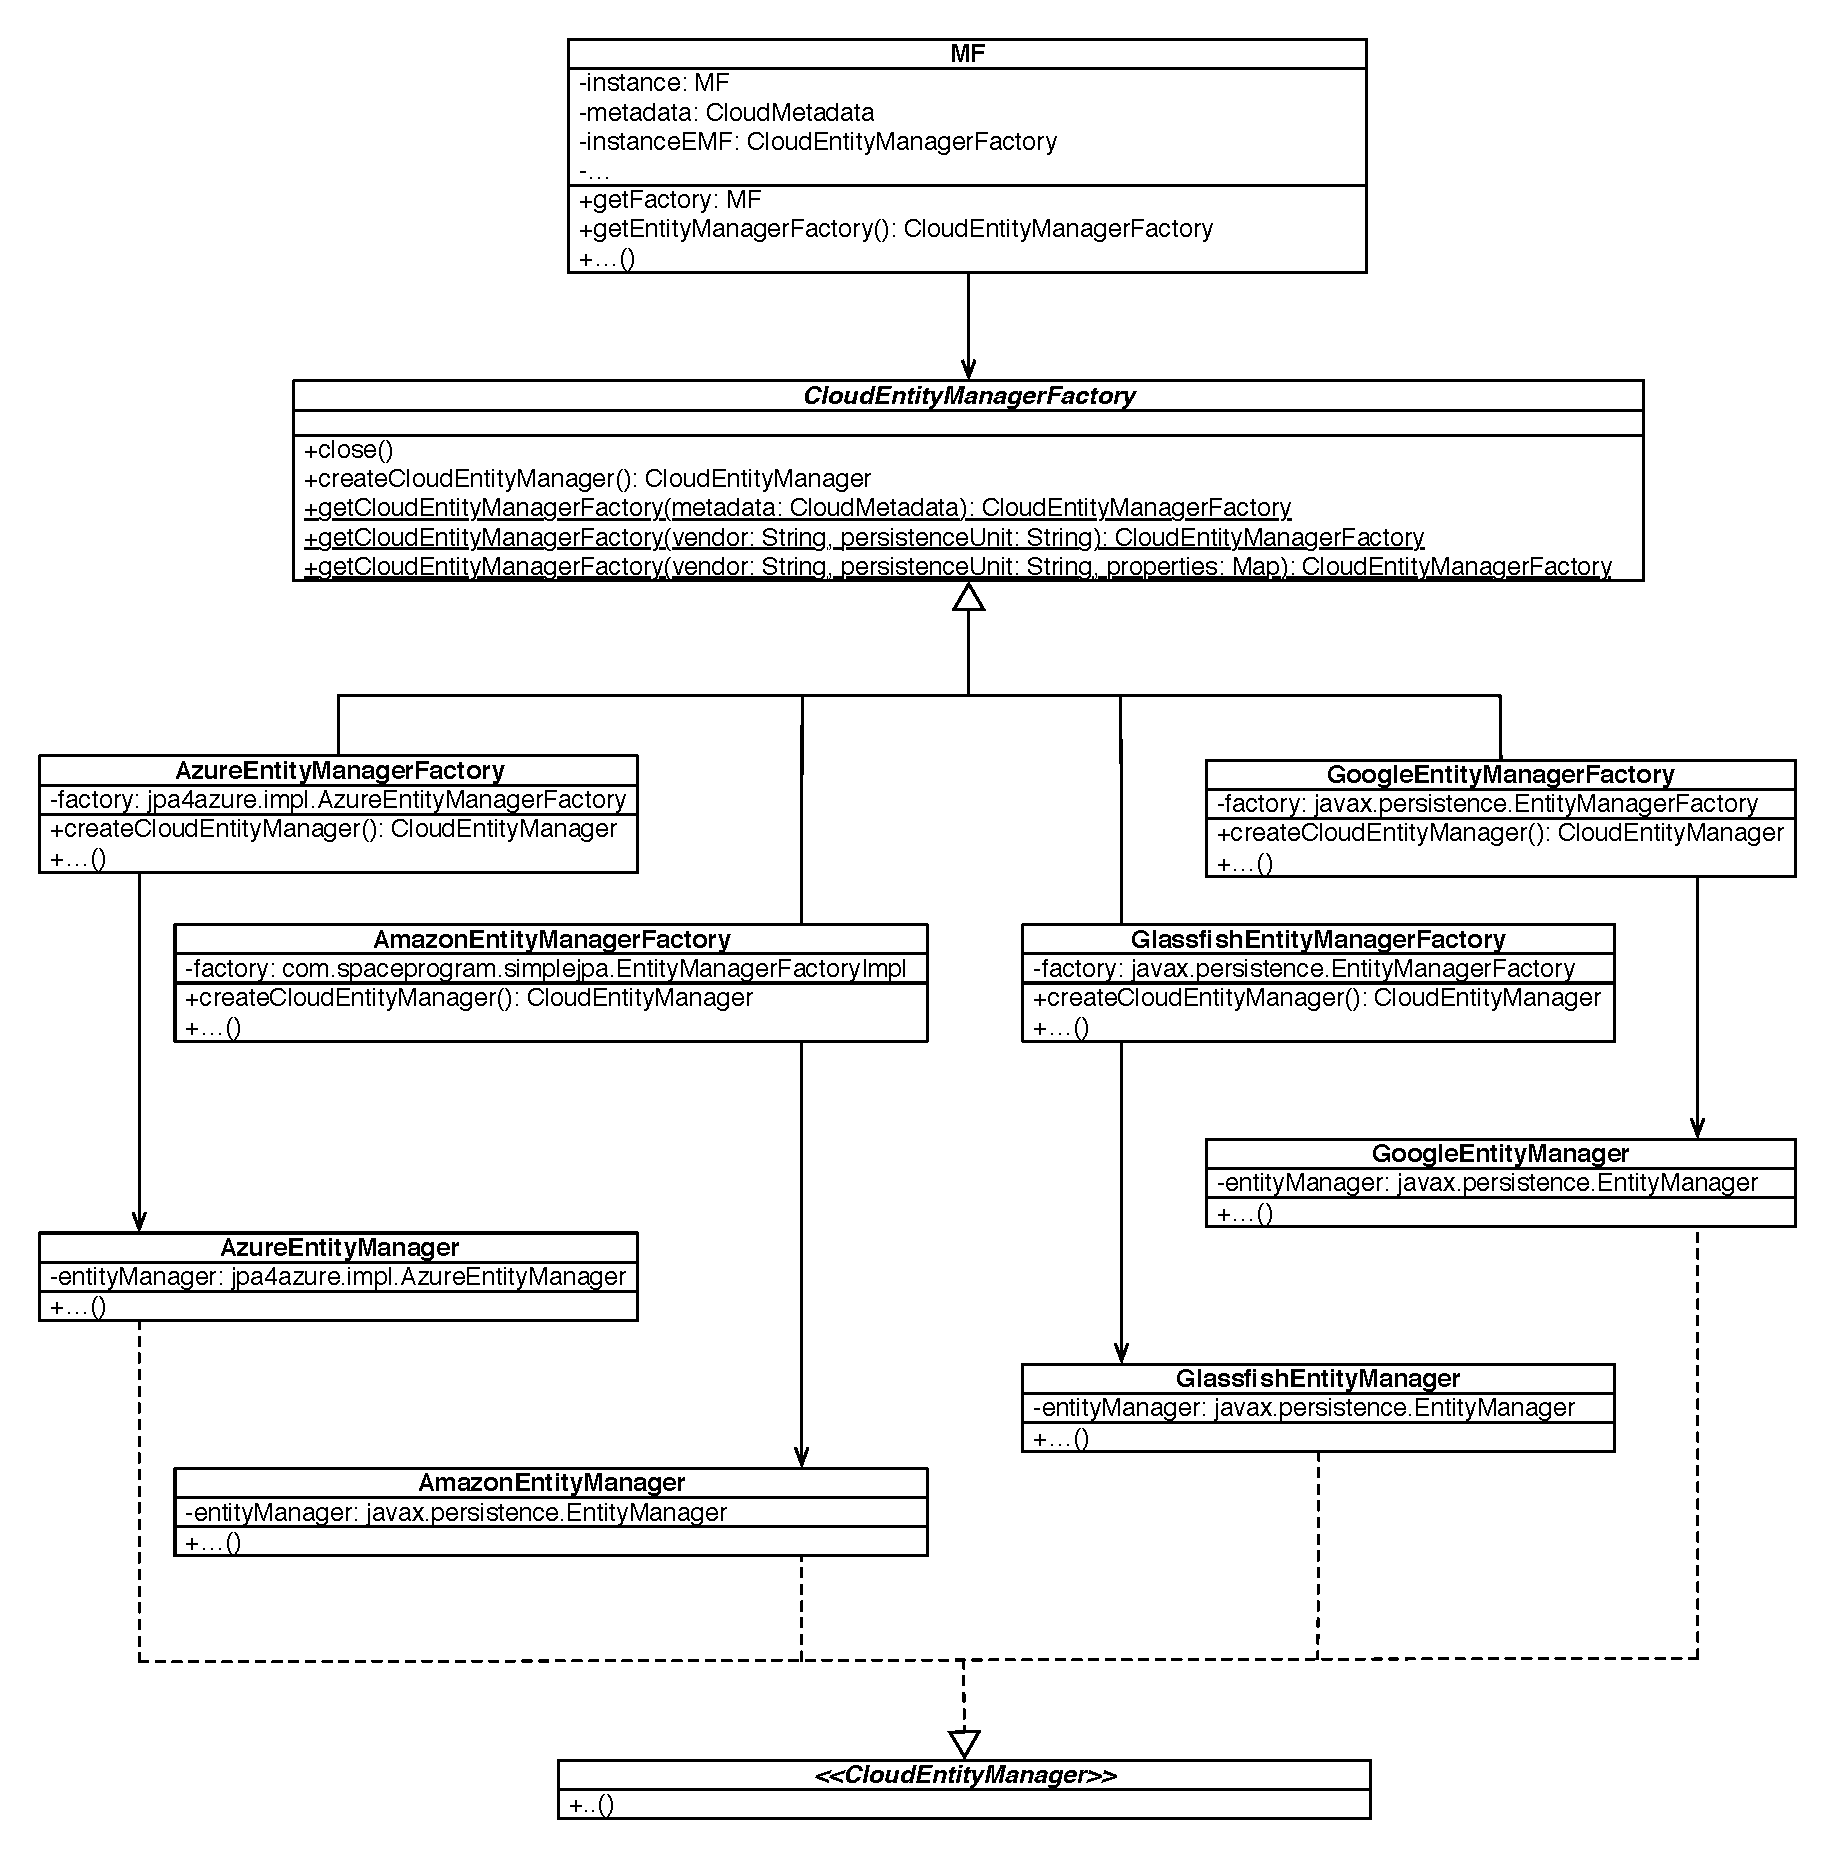
\includegraphics[width=14cm]{images/cpim_nosql_old}
  \caption{NoSQL service architecture}
  \label{fig:cpim-nosql}
\end{figure}

\noindent To use the service, the first step is instantiate a \texttt{CloudEntityManagerFactory} and, depending on the configuration file, this factory instantiate the vendor specific factory. For example in case that Google is the chosen vendor, the instantiated factory will be \texttt{GoogleEntityManagerFactory}. 
Each provider-specific \texttt{EntityManagerFactory} is responsible of instantiating an \texttt{EntityManager} which is the gateway to the underlying database. All the vendor-specific \texttt{EntityManager}(s) implement the common \texttt{CloudEntityManager} interface to achieve uniformity in methods and behavior.
The various implementation of the \texttt{CloudEntityManager} delegates every method call to the vendor-specific persistence provider. 

\newparagraph JPA is not a default language for NoSQL (as described in chapter \ref{chapter:sota}) but, due to its wide usage among Java developers, several JPA implementation has been build upon various NoSQL databases both developed by the vendor of the NoSQL storage or by the community.
This means that to support the NoSQL service through the JPA interface, an implementation of the JPA interface must be found. There are so three different persistence providers, one for each cloud provider:
\begin{itemize}
\item for \textit{Google Datastore} its used an official JPA implementation, available inside the SDK
\item for \textit{Amazon SimpleDB} its used \textbf{SimpleJPA}, a third-party implementation of the JPA interface
\item for \textit{Azure Tables} its used \textbf{jpa4azure}, a third-party implementation of the JPA interface
\end{itemize}

\noindent There are couple of things to notice: Amazon SimpleDB has been deprecated in favor of DynamoDB and \textit{jpa4azure} is not being maintained anymore, therefore CPIM needs to be updated in order to get rid of those outdated software.

\section{Kundera integration}
To solve this problems and reduce the number of software on which the CPIM rely on to provide the NoSQL service, the proposed solution  to modify the current CPIM architecture with a unique persistence provider that has been identified in Kundera.

\newparagraph The proposed solution is resumed in the architecture of figure \ref{fig:cpim-kundera} in which the benefit of having a single JPA provider are clearly visible. The architecture is slightly less articulated and no check on the selected provider is needed since this is handled by Kundera while reading the \texttt{persistence.xml} file in which the user will define what datastore is interested in.
Another benefit of this architecture is that the choice of the NoSQL technology is no more bound to the vendor specified in the CPIM configuration file, is in fact possible deploy the application in one of the supported PaaS provider and choose as NoSQL solution of another one which will be addressed remotely, simply by configuring the \texttt{persistence.xml}, moreover it's possible exploiting the Kundera polyglot persistency, to persist part of the data in a database and another part in another one defining the persistence units properly.

\begin{figure}[tbh]
  \centering
  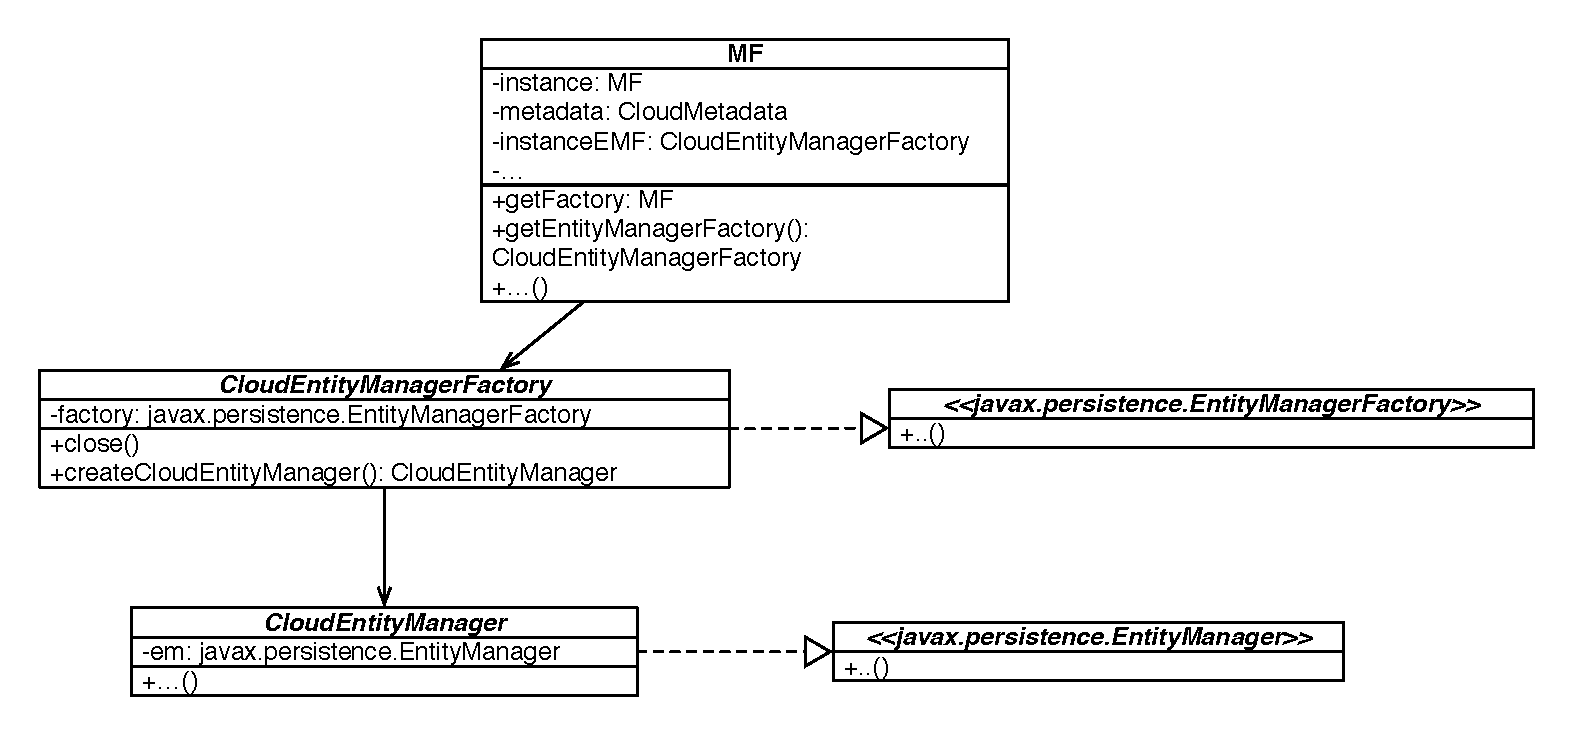
\includegraphics[width=14cm]{images/cpim_nosql_kundera}
  \caption{The modified NoSQL service architecture}
  \label{fig:cpim-kundera}
\end{figure}

\section{Hegira integration}
\label{sec:hegira}
\subsection{Intercepting CRUD operations}
\subsection{Intercepting queries}

\subsection{Build SQL statements}
\subsubsection{Build statements from objects}
\subsubsection{Build statements from JPQL queries}

\subsection{Migration Manager}
\subsubsection{Contacting the synchronization service}
\subsubsection{Handling the sequence numbers}
\section{Sending statements to Hegira}

\section{Summary}
